\section{Evaluation}\label{sec:eval}

We evaluate \name{}'s decentralized design and compare against a
state-of-the-art production workflow orchestrator---AWS Step Functions---on
latency and costs of running applications. Specifically, we ask the following
questions:

\begin{enumerate}

    \item Given the same application, i.e., the same user functions and the
    same workflow definition written as Step Functions, what is the end-to-end
    latency of running the application with \name{} after compiling it into
    \textit{unumized} functions and how does it compare with running it
    directly with Step Functions?

    \item What are the sources of \name{'s} latency overhead? How much does
    the overhead come from API calls to the underlying serverless components?

    \item Given the same application, what is the billing cost of running it
    with \name{} vs on Step Functions?

    \item What are the sources of \name{'s} billing costs? How much additional
    costs does the \name{} runtime incur in Lambda duration billing? And how
    much does it cost to provide exactly-once execution semantics from writing
    and reading checkpoints?

\end{enumerate}

% We show that 

% \begin{itemize}

%     \item over 97\% of \name{}'s latency overhead comes from API calls to
%     Lambda and data stores, which means the bulk of \name{}'s performance will
%     automatically improve with the underlying platform (e.g., a faster Lambda
%     or data store) without any modification to \name{} itself.

%     % \item The additional Lambda duration billing for executing \name{} runtime
%     % is negligible across all data sizes

%     \item \name{} is slightly faster (11-28\%) in chaining performance and
%     much faster in parallel fan-out and fan-in performance (up to 4.58x),
%     especially at higher level of parallelism, than Step Functions.

%     \item \name{} delivers more than one order-of-magnitude cost savings for
%     almost all applications we evaluated, even when using the more expensive
%     DynamoDB as the intermediary data store. The applications we use cover all
%     orchestration patterns that Step Functions currently support.

%     \item \name{} is able to express all orchestration patterns that Step
%     Functions currently support. Additionally, with the ExCamera
%     implementation, we demonstrate that \name{} can express fold or for loops
%     and support pipeline parallelism, neither of which is expressible in Step
%     Functions.

% \end{itemize}

\subsection{Experimental setup}

We use a set of microbenchmarks and 4 real-world applications in the
evaluation. The micro-benchmarks target basic orchestration patterns such as
chaining (\S\ref{sec:eval:chain}), fan-out and fan-in
(\S\ref{sec:eval:fan-out}), to gain insights into \name{}'s costs and latency
characteristics. We take the applications from serverless repositories and
prior research work, that encompass a variety of orchestration patterns, to
assess \name{}'s end-to-end performance and costs in real-world settings.

We run all experiments on AWS, region \texttt{us-west-1} and costs numbers
reflect \texttt{us-west-1} pricing. We configure lambdas to 128MB memory size
unless otherwise specified and use on-demand capacity mode for DynamoDB. To
avoid function cold starts, we pre-warm functions by running the workflow a
few dozen times before collecting data.

% S3 buckets all have Versioning turned on.

We compare against Step Functions as the baseline. All applications in the
evaluation are written as Step Functions state machines. For the Step
Functions experiments, we run the workflow definitions directly on AWS. For
the \name{} experiments, we first compile the Step Functions state machines to
unumized functions and then execute them as lambdas. The sole exception is
ExCamera due to limitations of the AWS State Language which we discuss in
\S~\ref{sec:eval:excamera}.

Step Functions experiments are executed using the \emph{Standard}
version~\cite{aws-step-functions-standard-vs-express}. Similar to \name{}, the
Standard workflows persist execution states on every state transition (i.e.,
completing one function and starting the next function), and always return
exactly one response for one workflow
invocation~\cite{aws-step-functions-exec-gntee}.

% We do not consider Step Functions' Express Workflows in our comparison because
% of its weaker execution guarantee, namely the same invocation could result in
% multiple and potentially diverging results if any part of the workflow logic
% is nonidempotent~\cite{aws-step-functions-exec-gntee}.

% Note that even though Step Functions claims that the Standard Workflows
% provides "exactly-once workflow
% execution"~\cite{aws-step-functions-exec-gntee}, it is not clear whether it
% implies exactly-once execution for component functions of the workflows. Our
% interpretation is that the internal states of a standard workflow will appear
% to execute exactly once, but component functions might not run exactly-once
% due to failures and retries, which is identical to \name{}. \shadi{this
% paragraph is a bit confusing... }

\subsection{Microbenchmarks}\label{sec:eval:micro}


\begin{figure}[t!]
    \centering
    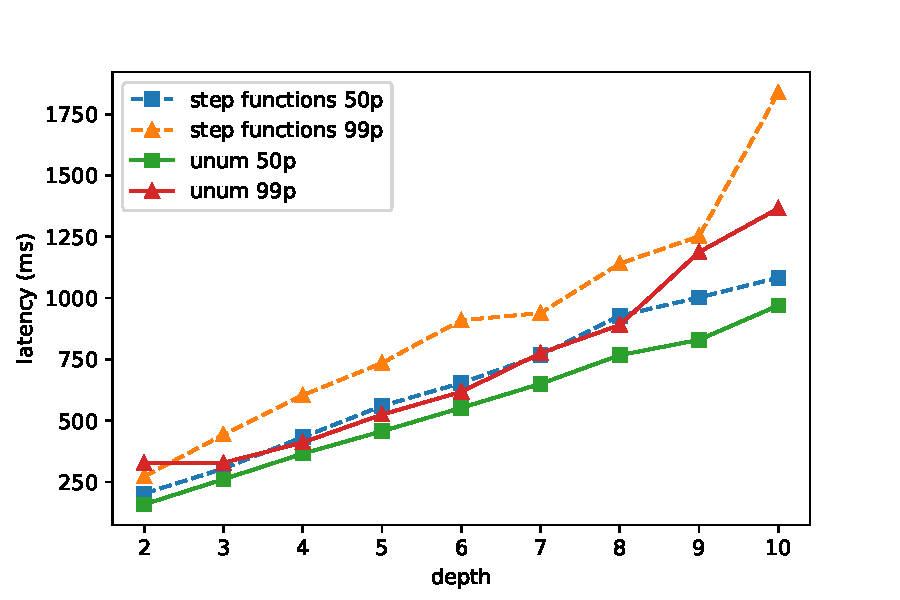
\includegraphics[width=\columnwidth]{figures/ChainMicroLatency.pdf}
    \caption{End-to-end latency of chaining N functions. All constituent
    functions in the experiment only run for 1-2ms, so the results mostly
    reflect the latency of the workflow systems. \name{} is marginally
    (11-28\%) faster than Step Functions on average. The results show that
    \name{} is basically as fast in the most fundamental orchestration
    primitive of transitioning from one function to the next.}
    \label{fig:chainmicrolatency}
\end{figure}

\begin{figure}[t!]
    \centering
    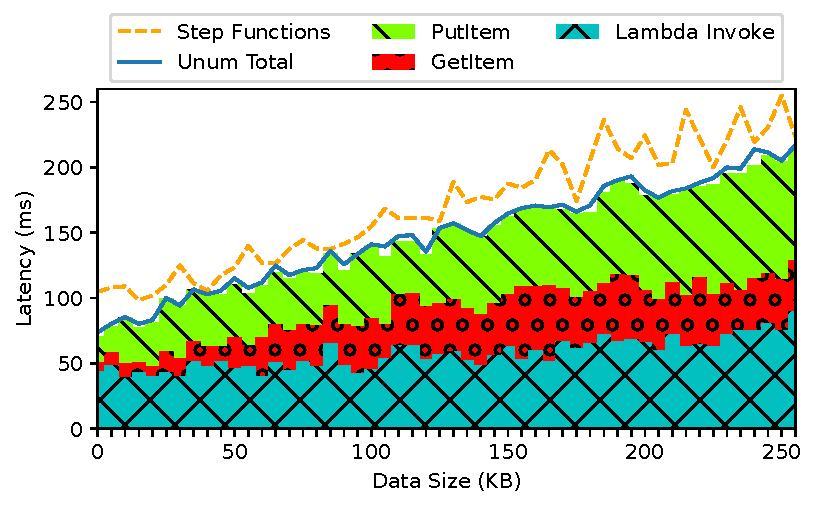
\includegraphics[width=\columnwidth]{figures/TotalAdditionalLatencyNBreakdown.pdf}
    \caption{\name{} latency of transitioning from the completion of a funtion
    to the start of the next function. The transition involves a Lambda
    invoke call, a checkpoint write to data store (a DynamoDB PutItem call)
    and a checkpoint read from data store (a DynamoDB GetItem call). Overall
    latency increases with data size due to more data written in the PutItem
    call and sent to next function via the Lambda invoke call. Over 97.5\% of
    the latency is the
    \name{} runtime waiting for data store accesses and Lambda invoke API
    calls to return. When the underlying platform improves (e.g., a faster
    Lambda or data store), the bulk of \name{}'s performance will
    automatically improve without any modification to \name{} itself.}
    \label{fig:single-transition-latency-breakdown}
\end{figure}

\begin{figure}[t!]
    \centering
    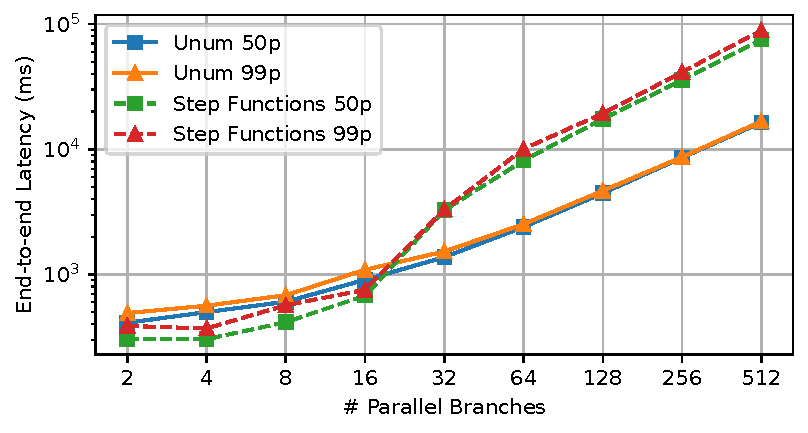
\includegraphics[width=\columnwidth]{figures/MapMicroLatency.pdf}
    \caption{End-to-end latency of parallel fan-out and fan-in with varying
    degrees of parallelism. All constituent functions in the experiment only
    run for 1-2ms, so the results mostly reflect the latency of the workflow
    systems. \name{} is around 100-200ms slower at lower degrees of
    parallelism (2-16 parallel branches), but starts to outperform Step
    Functions (2.37x faster) at even moderate parallelism level of 32 parallel
    branches. \name{}'s advantage widens as the the degress of parallelism
    increases, and is up to 4.58x at 512 parallel branches.}
    \label{fig:mapmicrolatency}
\end{figure}

\subsubsection{Chaining performance}\label{sec:eval:chain}

In this section, we evaluate how \name{} performs on executing a series of
steps in sequence, using the basic \texttt{chain} pattern, and compare with
Step Functions. We measure the end-to-end latency of executing a chain of
functions with varying chain length (2 to 10 functions). We want the
end-to-end latency to maximally reflects the performance of the workflow
system, and not the latency of user code. Therefore, we use a constituent
function that simply returns its input without any computations to keep the
user code runtime intentionally short (less than 2ms).

Figure~\ref{fig:chainmicrolatency} shows the end-to-end latency of Step
Functions and \name{} with DynamoDB. Overall, \name{} is around 43-173ms or
11-28\% faster in chaining than Step Functions. The slighly shorter latency is
likely because a transition in \name{} from one function to the next involves
a single network communication to Lambda when the source function calls the
target function asynchronously. On the other hand, in Step Functions, the same
transition first requires a network communication from the source function to
the orchestrator to send back the function output and then an invocation from
the orchestrator to Lambda. \name{} reduces the number of network
communications because control-flow states and logic are decentralized to
constituent functions and not managed by a centralized orchestrator.

\subsubsection{Single Transition Performance}

Using the same experiment from the last section, we further breakdown the
latency for \emph{a single transition} from one function to the next to
understand where the overhead of orchestration comes from. In \name{}, this
transition involves (1). the egress on the source function writing its output
to a checkpoint, (2). the egress on the source function invoking the target
function, and (3). the ingress on the target function checking whether a
checkpoint already exists to ensure exactly-once semantics. In total, that is
two storage accesses and one asynchronous invocation to Lambda. Because the
latency of storage accesses and Lambda invocation depends on the payload data
size, we measure across data sizes ranging between 0-255KB in 5KB
increments\footnote{Lambda limits payload size to 256KB for asynchronous
invocations.}.

Figure~\ref{fig:single-transition-latency-breakdown} shows the single transition
latency and its breakdown for \name{}. As a baseline, we also measure the same
latency of a state transition in Step Functions. However, Step Functions does
not generate fine-grained enough logs for a detailed breakdown. Overall,
\name{} is up to 56ms faster than Step Functions, likely for the same reason
of reduced number of network communications mentioned in the last section.

While the latency improvement is marginal, especially for workflows whose
functions perform real and expensive computations, \name{}'s latency breakdown
shows great potential for automatic future improvements as serverless gets
faster. Over 97.5\% of \name{}'s runtime overhead comes from APIs calls to the
underlying serverless systems, i.e., Lambda invocation, GetItem and PutItem
calls to DynamoDB. A faster NoSQL database or FaaS system will automatically
reduce bulk of \name{}'s latency without any modification to \name{} itself.


\subsubsection{Fan-out and fan-in performance}\label{sec:eval:fan-out}

Next, we evaluate how \name{} performs on executing a number of tasks in
parallel with the fan-out pattern, and compare with Step Functions. Quickly
launching parallel functions is important for serverless applications because
many require high degrees of parallelism (e.g., ExCamera runs thousands of
encoding lambdas in parallel) and migrate to serverless specifically for its
fast autoscaling.

We measure the end-to-end latency of launching a number of parallel branches
and then aggregating the result of all branches in a single fan-in function.
Similarly, we use a function that performs no computation so that the
end-to-end latency maximally reflects the performance of the workflow system.

\shadi{do we have any benchmarks with growing amount of computation in the
function itself?  or  a few representative datapoints.}\dhl{Not right now. Why
do you think this might be helpful? Using a short-lived function means the
numbers mostly measure the overhead of the system.}

Figure~\ref{fig:mapmicrolatency} shows the end-to-end latency (logscale) of
fan-out and fan-in at varying degrees of parallelism. At lower degree of
parallelism (2-16 parallel branches), \name{} is around 100-200ms or 26-32\%
slower than Step Functions. However, \name{} starts to outperform Step
Functions at even moderately higher parallelism of 32 parallel branches
(2.37x) and up to 4.58x at 512 parallel branches.

At lower degree of parallelism, \name{} is slower than Step Functions because
launching branches is slower with our Python implementation as the
asynchronous invocations essentially execute in series, while Step Functions
starts branches truly in parallel. However, Step Functions starts to throttle
branch creations very quickly. Step Functions documentation states that it
might pause creating branches when the number exceeds
40~\cite{aws-step-functions-map-state}, but we observe throttling starts
around 20 parallel branches. This explains why \name{} scales much faster when
the degree olf parallelism increases.

While our result is not arguing that centralized orchestrators fundamentally
scale worse than \name{}'s decentralized design, it is demonstrating that the
added orchestrator can easily become a performance bottleneck, whether due to
implementation or design restrictions, and its scalability problems has to be
solved again independently for the end-to-end system to perform well. On the
other hand, \name{} can leverage Lambda's fast autoscale capability without
imposing any additional restrictions because we introduce no new services and
build entirely on top of the existing serverless components.

% \subsubsection{Cost comparison}

% \begin{figure}[t!]
%     \centering
%     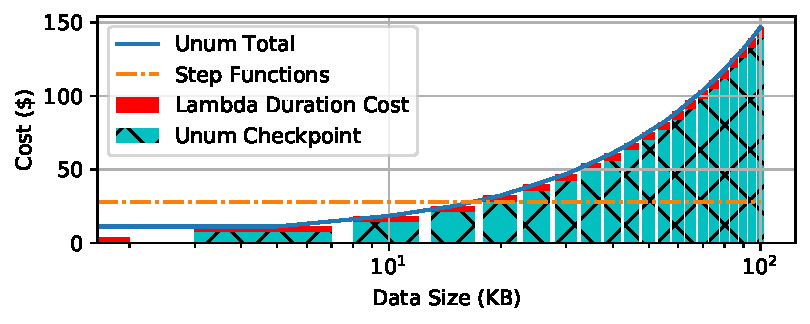
\includegraphics[width=\columnwidth]{figures/TotalCost.pdf}
%     \caption{Total costs comparison of 1 million state transitions between
%     Step Functions and \name{}. Computation assumes Lambda size of 3GB. \shadi{colors are hard to read}}
%     \label{fig:total-costs-single}
% \end{figure}

% \begin{figure}[t!]
%     \centering
%     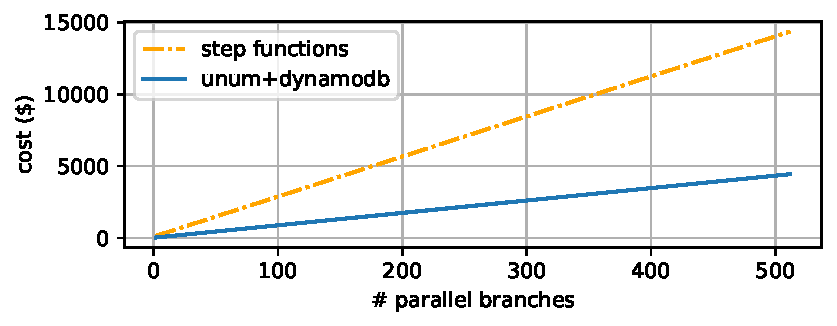
\includegraphics[width=\columnwidth]{figures/TotalMapCost.pdf}
%     \caption{Total costs comparison of fan-out and fan-in between Step
%     Functions and \name{}. Computation assumes Lambda size of 3GB and 1KB data
%     size for function outputs and checkpoints.}
%     \label{fig:total-costs-map}
% \end{figure}

% In this section, we break down the cost of running workflows with \name{} and
% compare with that of Step Functions. We discuss the costs for a single transition,
% chaining and fan-out.

% Costs numbers are calculated based on AWS pricing for \texttt{us-west-1}
% region. We do not "measure" the cost of running workflows because AWS does not
% provide real-time billing data. We scale costs numbers by 1 million to ease
% reading.

% Step Functions charges based on the number of state
% transitions~\cite{aws-step-functions-pricing}. Each state transition is charged
% a fixed rate of \$27.9 $ \times 10^{-6}$.

% There are two parts to \name{}'s costs: (1). additional Lambda duration
% billing for running the \name{} runtime, and (2). data store reads and writes.

% We do not count the storage costs in the intermediary data store because after
% a workflow execution, checkpoints can be immediately deleted or moved to
% cheaper storage by the user.

% Figure~\ref{fig:total-costs-single} shows the total cost of transitions for
% function data size varying between 0-255KB. The computation assumes Lambda
% memory size of 3GB. We can see that the additional Lambda duration costs from
% running \name{} runtime is a small fraction when compared with the costs of
% DynamoDB writes. \shadi{how is the figure showing this? how do you translate lambda duration to cost in the figure? this figure is hard to understand. }
% In fact, even at 255KB, the additional Lambda
% duration costs is only abour \$10. If using the smallest 128MB lambdas \shadi{(instead of 3GB)}, the
% costs diminishes to merely \$0.46.

% DynamoDB writes dominates the costs in \name{} because the on-demand mode
% charges only not on the number of writes but also on the amount of data
% written. For 1KB of data, DynamoDB charges $1.3942 \times 10^{-6}$ for a write
% and $0.279 \times 10^{-6}$ for a read. Because checkpoint reads do not return
% any data when there are no faults, the cost of checkpoint reads does not
% increase with the data size and stays merely \$0.279 for the computation in
% Figure~\ref{fig:total-costs-single}.

% Even though the simulation in Figure~\ref{fig:total-costs-single} shows the
% costs of \name{} outpacing that of Step Functions at larger data sizes, our
% macrobenchmark results demonstrate that functions in real-world serverless
% workflows do not output large amount of data. In fact, workflows tend to use
% their own storage and manage application data manually. Checkpoints in the
% \name{} intermediary data store are normally under 1KB. 

% Figure~\ref{fig:total-costs-map} shows the total costs of fan-out and fan-in
% when function checkpoints are under 1KB. In addition to the costs discussed
% for a single transition, the entry function performing the fan-out incurs
% higher Lambda duration costs for invoking each fan-out function. The fan-in
% function at the end also causes extra costs because it reads the checkpoints
% of all fan-out branches. However, the total costs of this microbenchmark is
% more than 3.2x lower with \name{} than Step Functions.

% \begin{itemize}

%     \item S3 charges \$5.5 per 1M PUT requests (for checkpoint write) and \$0.44
%     per 1M GET requests (for checkpoint read).

%     \item DynamoDB on-demand capcity mode charges reads and writes based on
%     the data size. 1M requests for writing 1KB data costs \$1.3942 and 1M
%     requests for reading 1KB data costs \$0.279. Note that in the case of
%     DynamoDB, if no faults happen during execution, the checkpoint read will
%     return "item not found", which costs the same as returning 1KB of data.

%     \item For 1M state transitions, \name{}'s costs for S3:

%     \[  r(d)\times0.05 + 5.94 \]

%     and for DynamoDB:

%     \[  r(d)\times0.05 + d\times1.3942 +0.279\],

%     where $r$ is the total additional runtime of \name{}, $d$ is the data
%     size.

% \end{itemize}




\subsection{Real-World Applications}

% \begin{table}[]
% \begin{tabular}{llllll}
% \hline
%                      &                        & \multicolumn{2}{l}{\textbf{unum}}                                                                                                   & \multicolumn{2}{l}{\textbf{Step Functions}}                                                                     \\
% \textbf{Application} & Pattern                & \textit{e2e latency} & \textit{cost (per 1M exec.)}                                                                                 & \textit{e2e latency} & \textit{cost (per 1M exec.)}                                                             \\ \hline
% IoT Pipeline         & chain                  & 120.9ms              & $0.2*2+(73+28)*$0.0021+2*\$1.3942                                                                            & 226.52               & $0.2*2+ 4*$27.9                                                                          \\
% Text Processing      & fan-out, fan-in        & 562.69ms             & $0.2*6+ (105+149+70+68+144+100)*$0.0021 + 6*$1.3942+2*2*$0.279                                               & 552.46ms             & $0.2*5+7*$27.9                                                                           \\
% Wordcount            & chain, fan-out, fan-in & 410s                 & $0.2*(1+262+1+250+1) + (277+6264*262 + 348 + 667*250 +68)*$0.0021 +(1+262+1+250+1)*$1.3942 + 262*2*$0.279+ 250*2* $0.279    & 898s                 & $0.2*(1+262+1+250+1) + (5913*262 + 154 + 633*250 +5)*$0.0021 +(1+262+1+1+250+1+1)*\$27.9 \\
% ExCamera             & chain, fan-out, fold   & 84s                  & $0.2*(1+16+15+15+14) + (6500+1500+350+4500+5000)*$0.0021+ (1+16+15+15+14)*$1.3942 + 15*2*$0.279+14*2*\$0.279 & 98s                  & $0.2*(16+16+1+16+15)+(6300+1400+2+5500+5300)*$0.0021+(1+16+16+1+1+16+1+1)*\$27.9      \\ \hline
% \end{tabular}
% \end{table}

\begin{table*}[t]
\centering
\begin{tabular}{ll|rr|rr}
\hline
                     &                        & \multicolumn{2}{c}{\textbf{Latency (seconds)}}            & \multicolumn{2}{c}{\textbf{Cost (\$ per \emph{1 mil.} executions)}}       \\
\textbf{Application} & \textbf{Pattern}       & \textit{\name{}} & \textit{Step Functions}   & \textit{\name{}} & \textit{Step Functions}            \\ \hline
IoT Pipeline         & chain                  & 0.18       & 0.23       & 3.4       & 111.6   \\
Text Processing      & fan-out, fan-in        & 0.56       & 0.55       & 12.0      & 196.3   \\
Wordcount            & chain, fan-out, fan-in & 410.64     & 898.56     & 4,904.8   & 18,113.0 \\
ExCamera             & chain, fan-out, fold   & 84.17      & 98.42      & 8,299.5   & 84,150.0      \\ \hline
\end{tabular}
\caption{Latency and costs comparison between \name{} and Step Functions for
the macrobenchmark applications. Running applications on \name{} is 3.7x to
32.8x cheaper than on Step Functions. Furthermore, \name{} is faster than Step
Functions especially for workflows with high degrees of parallelism. Text
Processing is the only workflow which \name{} is marginally slower because
Step Functions creates parallel branches faster at low fan-out degrees as we
illustrated in Figure~\ref{fig:mapmicrolatency}.}
\label{table:macro}
\end{table*}

\begin{table}[]
\centering
\begin{tabular}{|r|r|}
\hline
                                  & \textbf{Latency (seconds)} \\ \hline
\textbf{Original ExCamera}        & 76                         \\ \hline
\textbf{gg}                       & 90                         \\ \hline
\textbf{\name{}} & 84                         \\ \hline
\end{tabular}
\caption{\name{}'s implementation closely matches that of gg and the original
ExCamera where a task starts as soon as its input data becomes available. The
Step Functions implementation had to serialize the encoding and re-encoding
stages because the \texttt{Map} state in Step Functions requires all parallel
branches to complete before fan-in.}
\label{table:excamera}
\end{table}

In this section, we evaluate \name{}'s performance and costs with 4 real-world
workloads and compare with Step Functions. We use the following applications
taken from serverless applications repositories and prior research work. The
applications cover a range of use cases and workflow patterns:

\begin{itemize}
    \item \textbf{IoT Pipeline} Adapted from a humidity control application in the
    AWS serverless repository~\cite{iot-pipeline}. The workflow consists of a
    chain of two functions where the first function processes time-series data on
    indoor climate and outputs a set of aggregate statistics. The second function
    makes a HVAC system control decision based on the statistics and adjusts the
    HVAC settings.

    \item \textbf{Text Processing} Adapted from the social networks application in
    the DeathStarBench~\cite{deathstar}. The workflow consists of 5 functions that
    create a social network post by processing text data of user posts. It fans
    out to two branches that resolves user mentions and shortens URLs in parallel.
    Eventually, it fans in to a function that saves the post along with resolved
    user mentions and shortened URLs in a NoSQL database.

    \item \textbf{Wordcount} Adapted from MapReduce word count~\cite{mapreduce}.
    Mappers and reducers execute as Lambda function. The workload uses 250
    parallel mappers and reducers.

    \item \textbf{ExCamera} ExCamera~\cite{excamera} is a novel video encoder that
    encodes large raw videos with thousands of parallel functions to achieve
    low latency. The workflow consists of three stages, \texttt{ENCODE},
    \texttt{ENCODE-GIVEN-STATE} and \texttt{REBASE}, where functions interact
    in complex patterns. The first stage is a \texttt{map} that runs many
    \texttt{ENCODE} functions entirely in parallel, the second stage forms
    paralllel pipelines following the first stage where the $i^{th}$
    \texttt{ENCODE-GIVEN-STATE} branch starts when the $(i)^{th}$ and
    $(i-1)^{th}$ \texttt{ENCODE} branch complete. The final \texttt{REBASE}
    runs in series and rebases each chunk on top of the state from the
    previous chunk.

    We implement a \name{} version and Step Functions version for ExCamera,
    using the same binaries in constituent functions as the original
    paper~\cite{excamera-binary}. The \name{} implementation closely matches
    the original ExCamera where a task starts as soon as its input data
    becomes available. But the Step Functions implementation had to serialize
    the \texttt{ENCODE}, \texttt{ENCODE-GIVEN-STATE} stages because fan-outs
    in Step Functions require all parallel branches to complete before fan-in.
    For this reason, we do not derive the \name{} version from a Step
    Functions definition with the frontend compiler. Instead, we hand-write
    \name{} configurations for each constituent function.

    Furtheremore, we compare \name{}'s implementation against the original
    authors' implementation of ExCamera. The original authors build two
    version: a hand-optimized version in the original paper implemented with
    the \texttt{mu} framework which exposes a state machine abstraction, and a
    later version implemented with the \texttt{gg} framework which uses a
    thunk abstraction. We use the exact same workload and setup as the
    experiment in \texttt{gg}~\cite{gg-atc}, i.e., the same input video of the
    first 888 chunks of \texttt{sintel-4k} video, 16 chunks per batch and
    lambdas with 3GB of memory.

\end{itemize}

\subsubsection{Latency Comparison}

Table~\ref{table:macro} compare the median end-to-end latency and costs (per 1
million executions) of running the applications with \name{} and with Step
Functions. Similar to our results in microbenchmarks (\S\ref{sec:eval:micro}),
\name{} is around 50ms or 27.8\% faster in the chaining application---IoT
Pipeline, and 2.2x faster in the highly-parallel application --- wordcount.
Text Processing is the only application where \name{} is slower than Step
Functions. We know from \S\ref{sec:eval:fan-out} that \name{} is around 100ms
slower launching 2 parallel branches. However, with constituent functions
performing real computation and chaining of function in parallel branch,
\name{}'s end-to-end latency is merely 10ms or 1.8\% slower than Step
Functions.

While ExCamera process all 888 chunks in parallel, each batch is a
\texttt{map} with only 16 branches. From the result in
\S\ref{sec:eval:fan-out}, we know that \name{} is around 200ms slower than
Step Functions when launching 16 parallel branches. However, \name{} is able
to win back 14.24s or 17\% of latency performance because fan-in in \name{} is
wait-free. \name{} invokes the fan-in function whenever its input becomes
available, whereas Step Functions first requires all branches to complete even
if a branch is not part of the fan-in function's input, and lacks programming
constructs to express fine-grained data dependencies between branches that can
enable ``partial fan-in''.

\dhl{Explain the difference between unum fan-in and Step Functions fan-in in
design already. Specifically, unum fan-in starts when all inputs are
available, whereas Step Functions fan-in first requires all branches to
complete even if a branch is not part of the fan-in function's input.}

Table~\ref{table:excamera} compares \name{}'s implementation of ExCamera with
the original implementation and \texttt{gg}'s version. \name{}'s is 7.1\%
faster than gg and \%10.5 slower than the original ExCamera. The original
ExCamera pre-loads raw video chunks into lambdas before starting, while
\name{} and \texttt{gg} do not. The original authors attributes the
comparatively slower performance of \texttt{gg} to the lack of pre-loading
which is likely also the reason for \name{}'s slower performance. But
different from \texttt{gg}, \name{} executes control-flow logic in a
decentralized manner while \texttt{gg} has a centralized coordinator on EC2
that proxies inter-function communications and invokes lambdas. The reduced
number of network communications likely explains why \name{} is slightly
faster than \texttt{gg}.

\subsubsection{Cost Comparison and Breakdown}

\begin{figure}[t!]
    \centering
    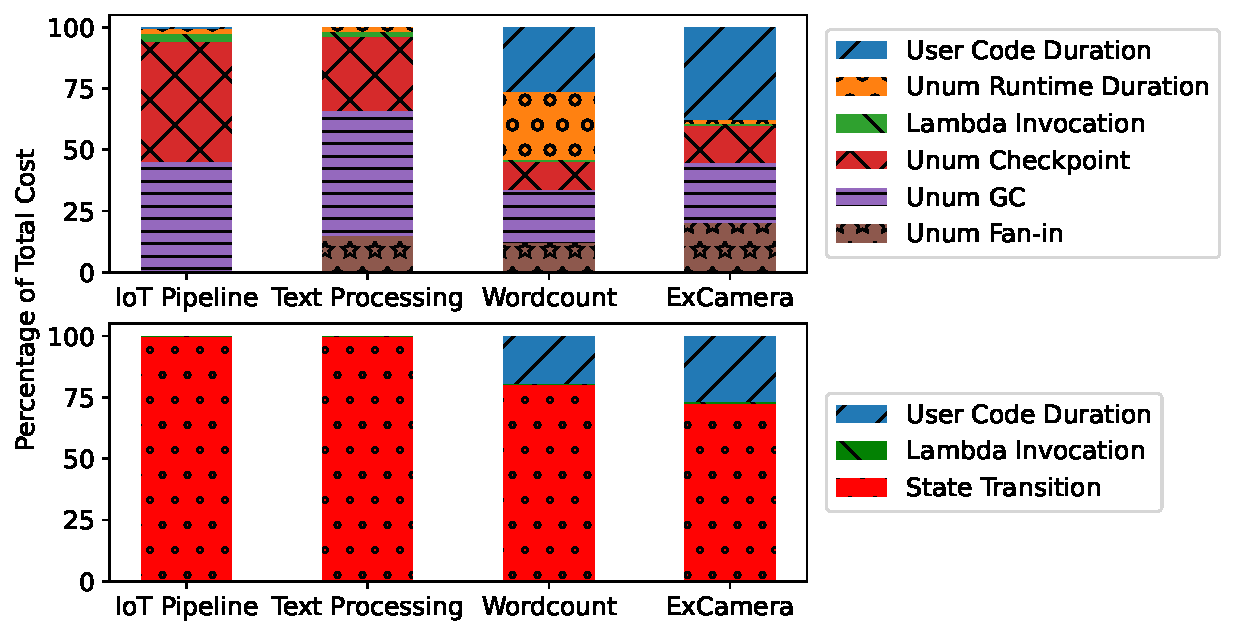
\includegraphics[width=\columnwidth]{figures/AppCostBreakdown.pdf}
    \caption{TODO}
    \label{fig:cost-breakdown}
\end{figure}

Moreover, \name{} is consistently cheaper than Step Functions for all
workloads with up to 32.8x costs savings. All costs numbers in
Table~\ref{table:macro} are calculated based on public pricing information for
AWS \texttt{us-west-1} region. We do not ``measure'' the costs of running
workflows because AWS does not provide real-time billing results for all
services.

For Step Functions, the total costs of running an application consists of i.
Lambda duration billing for running user code, ii. Lambda invocation billing
for starting functions and iii. Step Functions state transition
charges~\cite{aws-step-functions-pricing}. Step Functions charges a fixed rate
of \$27.9 $ \times 10^{-6}$ per state transition. A state transition equates
to an edge in the workflow graph in the case of chaining and fan-out. But
fan-in only counts as one state transition. Additionally, Step Functions adds
a \texttt{Start} and \texttt{End} state to each workflow that counts towards
state transitions.

The total costs of running an application with \name{} consists of i. Lambda
duration billing for running the \emph{unumized} functions, that is both the
user code and \name{} runtime code, ii. Lambda invocation billing for starting
functions, and iii. data store reads and writes for checkpoints. DynamoDB
charges $1.3942 \times 10^{-6}$ for writing and $0.279
\times 10^{-6}$ for reading 1KB of data. We do not count the costs of storing
the data in DynamoDB because after a workflow execution, users can immediately
delete the checkpoints or move them to cheaper storage.

Figure~\ref{fig:cost-breakdown} shows the cost breakdown for 



\dhl{Sync with Intro, if we say anything about billing schemes or predicted
cheaper costs.}

% \subsubsection{Questions}

% \begin{enumerate}

%     \item How do we evaluate and present execution guarantee? Anything to show
%      to convince our reader that it's correct?

%     \item How do we evaluate other benefits that stem from a simpler design
%      (the fact that unum gets rid of the needs for a separate orchestrator
%      service), such as resource management, required staffing and other
%      hosting costs? Further on the resource utilization point, do we want to
%      say that dollar costs of running applications is a reasonable enough
%      proxy to resource consumption and therefore lower price = less resource
%      consumption = better resource utilization?

%     \item Should we run experiments with S3 and present those numbers?

%     \item How to discuss the expressiveness advantage? Specifically,

%         Step Functions has no way to express a for loop or fold.

%         Step Functions has no way to express pipeline parallelism.

%         Step Functions fan-in needs to make sure the aggregate data doesn't exceed a
%         limit, unum automatically passes data in using pointers to the intermediary
%         data store.

% \end{enumerate}

